\documentclass[11pt,a4paper]{article}
\usepackage{hw}
\usepackage{subcaption}

\graphicspath{ {.} }
\setlength\parindent{0pt}

\begin{document}
\qtitle{Ex1}
Let $H=rect(2x/\pi)$, for $C\rightarrow D$, $g=[g_1, g_2, ..., g_k]$ while $g_k(x)=H_kf(x)=\bint{-\infty}{\infty} rect(2(x-x')/\pi) cos(2x')sin(x'/4)dx'$. 

Then the adjoint of $H$ is $H^*=\overline{rect(2x/\pi)}$, $H^*g(x)=\sum_k \overline{rect(2x/\pi)}g_k$. 

We set x discrete interval to 0.01.

\begin{lstlisting}
import numpy as np
import matplotlib.pyplot as plt

# EX1 
xlim = 50
expand = 20
x = np.linspace(-xlim, xlim, expand*xlim+1)
x_inter = 2*xlim/(expand*xlim+1)
print("x interval: ", x_inter)
# f
f = np.cos(2*x) * np.sin(x/4)
# rect kernel
rect = np.zeros_like(x)
rect_half_w = 1/np.pi
start_rect_idx = int((xlim-rect_half_w) // x_inter)
end_rect_idx = int(len(x) - start_rect_idx)
rect[start_rect_idx:end_rect_idx] = 1

# convolve 
image = np.convolve(f, rect, mode="same") / np.sum(rect)

# display value in range [0, 8pi]
disp_start, disp_end = int(len(x)//2), int(len(x)//2 + 8*np.pi/x_inter)
fig = plt.figure()
# object 
plt.plot(x[disp_start:disp_end], f[disp_start:disp_end], label="object f(x)")
# image
plt.step(x[disp_start:disp_end], image[disp_start:disp_end], label="image Hf(x)")
plt.step((x[disp_start], x[disp_end]), (0, 0), "k--")

# H*g
hg = np.convolve(image, rect, mode='same') / np.sum(rect)
# check <Hf, g> = <f, H*g>
inner1 = np.sum(image*image)
inner2 = np.sum(hg*f)
assert inner1 == inner2

plt.step(x[disp_start:disp_end], hg[disp_start:disp_end], label="H*g")

plt.legend()
plt.xlabel("x")
plt.xlim(x[disp_start], x[disp_end])
plt.show()
\end{lstlisting}

The results are shown as Fig.~\ref{fig:ex1}.

\begin{figure}
    \centering
    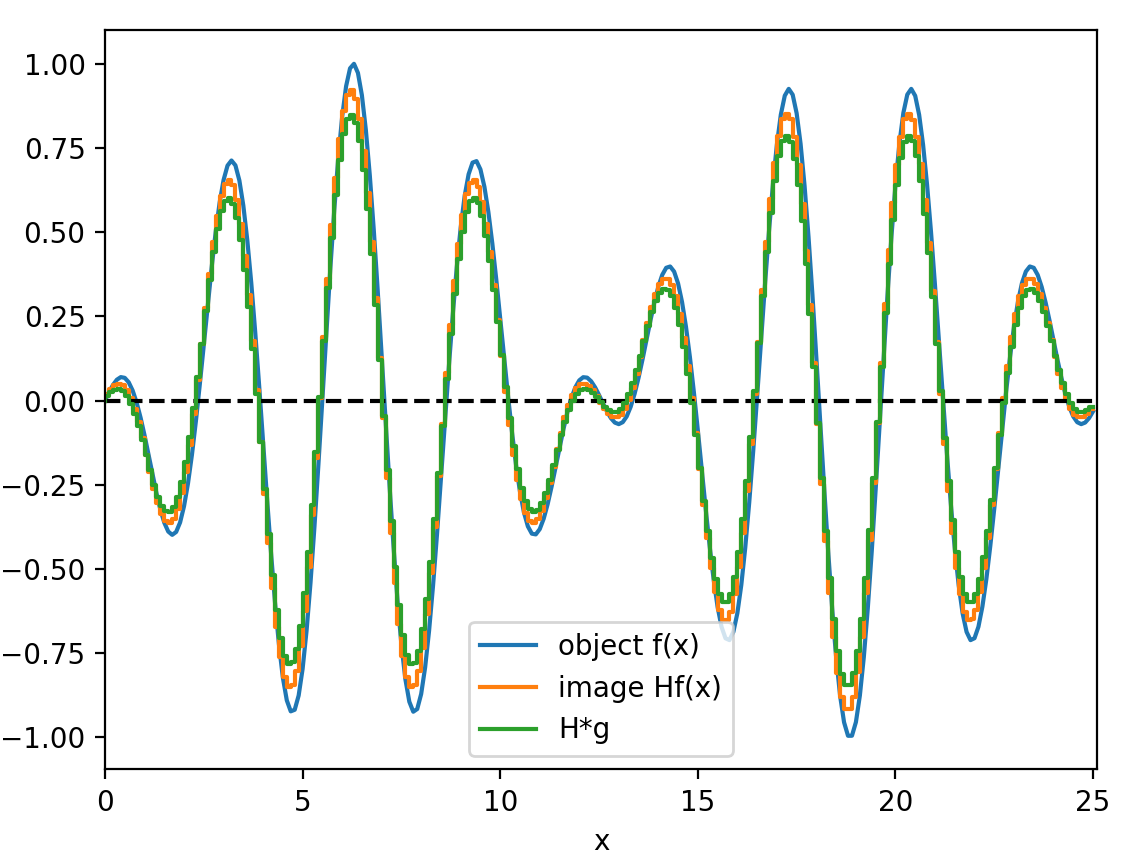
\includegraphics[width=\linewidth]{HW2_Q1_1.png}
    \caption{Result figure of object f, image g, and $H^*g$}
    \label{fig:ex1}
\end{figure}

\newpage
\qtitle{Ex2}
Let $H=rect(x/a)$ and $f=rect(x/a)$,\\
$g=Hf=\bint{-\infty}{\infty}rect((x-x')/a)rect(x'/a)dx'=\bint{-a/2}{a/2}rect((x-x')/a)dx'$.
 
So to make $rect((x-x')/a)=1$, $-a/2<x-x'<a/2\rightarrow x-a/2<x'<x+a/2$. 

If $x\in [-3a/2, -a/2]$, $-a/2<x+a<a/2$. $g=(x+a)-(-a/2)=x+3a/2$. 

Otherwise, when $x\in[-a/2,a/2]$, $a/2<x+a<3a/2$. $g=a/2-x$

\newpage
\qtitle{Ex3}
\textbf{a.}

\begin{lstlisting}
R = 64
C = 64
image = np.zeros((R, C))
image[R//2, C//2] = 64
image[R//4, C//4] = 128

# number of views
N = 256
theta = np.linspace(0, 180, N)
sinogram = radon(image, theta=theta)
plt.imshow(sinogram)
plt.show()
\end{lstlisting}

\begin{figure}[!ht]
    \centering
    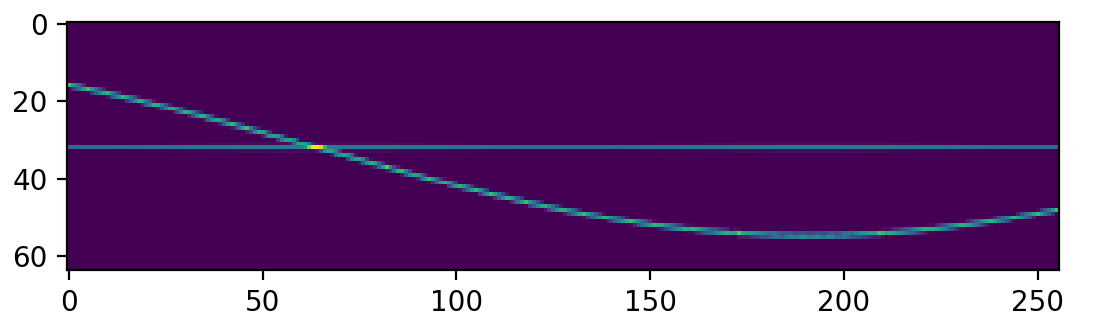
\includegraphics[width=\linewidth]{HW2_Q3_1.png}
    \caption{Sinogram of image $f(r,c)$}
\end{figure}

\textbf{b.}

\begin{lstlisting}
    from scipy.signal import peak_widths

    recon_image = iradon(sinogram, theta=theta, filter_name=None)
    # estimate none-zero area
    nonzero = recon_image.copy()
    nonzero[nonzero > 0] = 1
    # recon value error 
    pt1_err = recon_image[R//2, C//2] - image[R//2, C//2]
    pt2_err = recon_image[R//4, C//4] - image[R//4, C//4]
    # max error of other non-zero region 
    diff = np.abs(recon_image - image)
    diff[R//2, C//2] = 0
    diff[R//4, C//4] = 0
    pt1_profile = recon_image[R//2, :]
    pt2_profile = recon_image[R//4, :]
    pt1_w = peak_widths(pt1_profile, np.array([R//2]))
    pt2_w = peak_widths(pt2_profile, np.array([R//4]))
    print("Peak width: ", pt1_w, pt2_w)
    print("Error between original object and reconstructed object: ", pt1_err, pt2_err)
    print("Other non-zero region error: \{\}", np.max(diff))
    \end{lstlisting}

\begin{figure}[!ht]
    \centering
    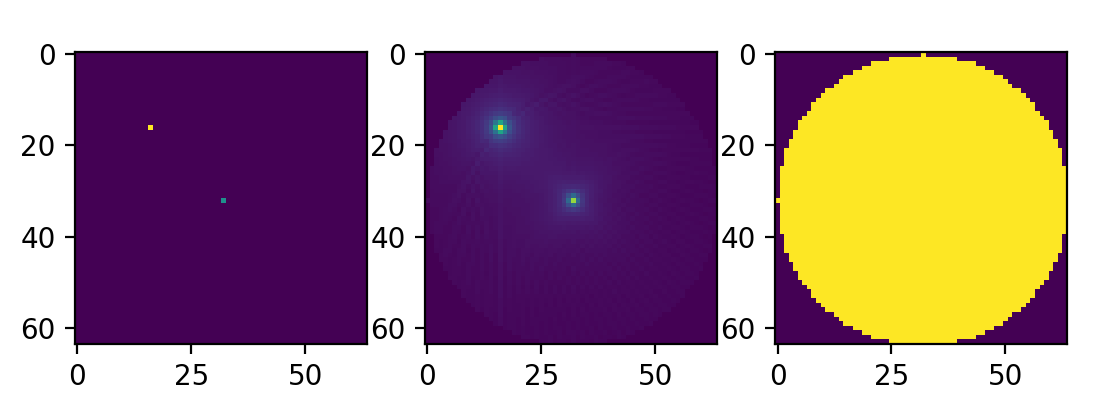
\includegraphics[width=\linewidth]{HW2_Q3_2.png}
    \caption{Left: original object image $f(r,c)$; middle: reconstructed object image $\widehat{f(r,c)}$; right: yellow region indicates the non-zero region in the reconstructed object image $\widehat{f(r,c)}\ne 0$.}
\end{figure}

The error between the two points on the original object and the reconstructed object is 48.31 and 5.64, respectively. Apart from the two points, other non-zero region in the reconstructed object image contains error up to 78.78, with mean error as 4.48. Therefore, it seems to be not a perfect estimate of $f(r, c)$

\newpage
\textbf{c.}
\begin{figure}[!htp]
    \centering
    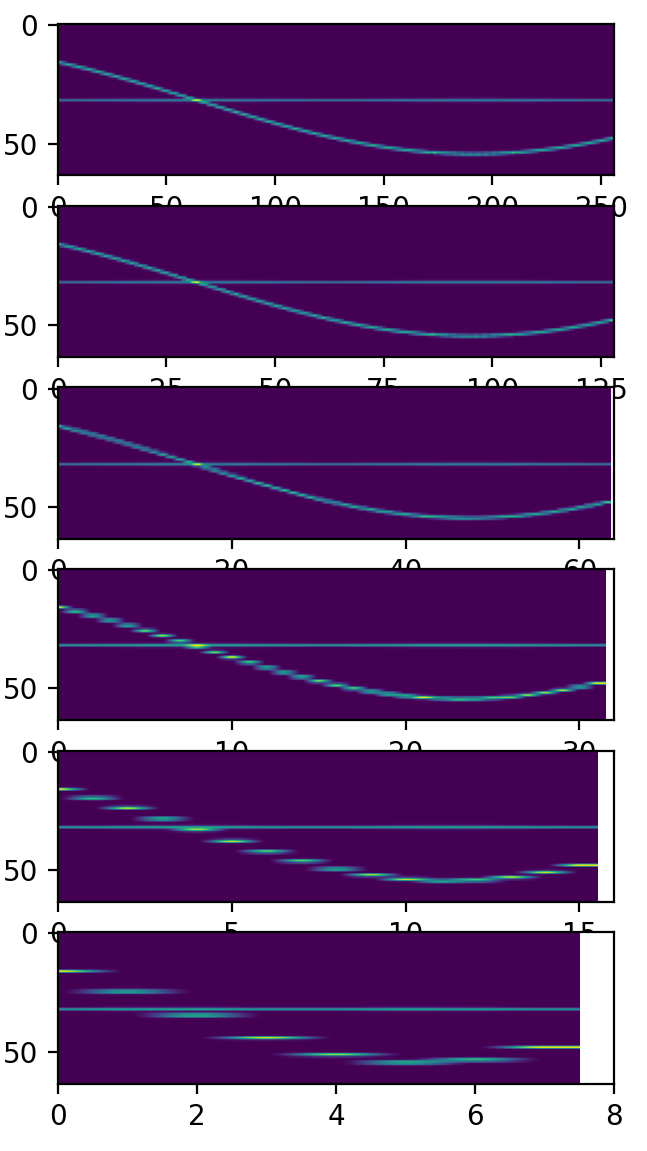
\includegraphics[width=0.7\linewidth]{HW2_Q3_3.1.png}
    \caption{Sinograms of N from 256 to 8 (Top to bottom).}
    \label{fig:sino}
\end{figure}

\begin{figure}[!htp]
    \centering
    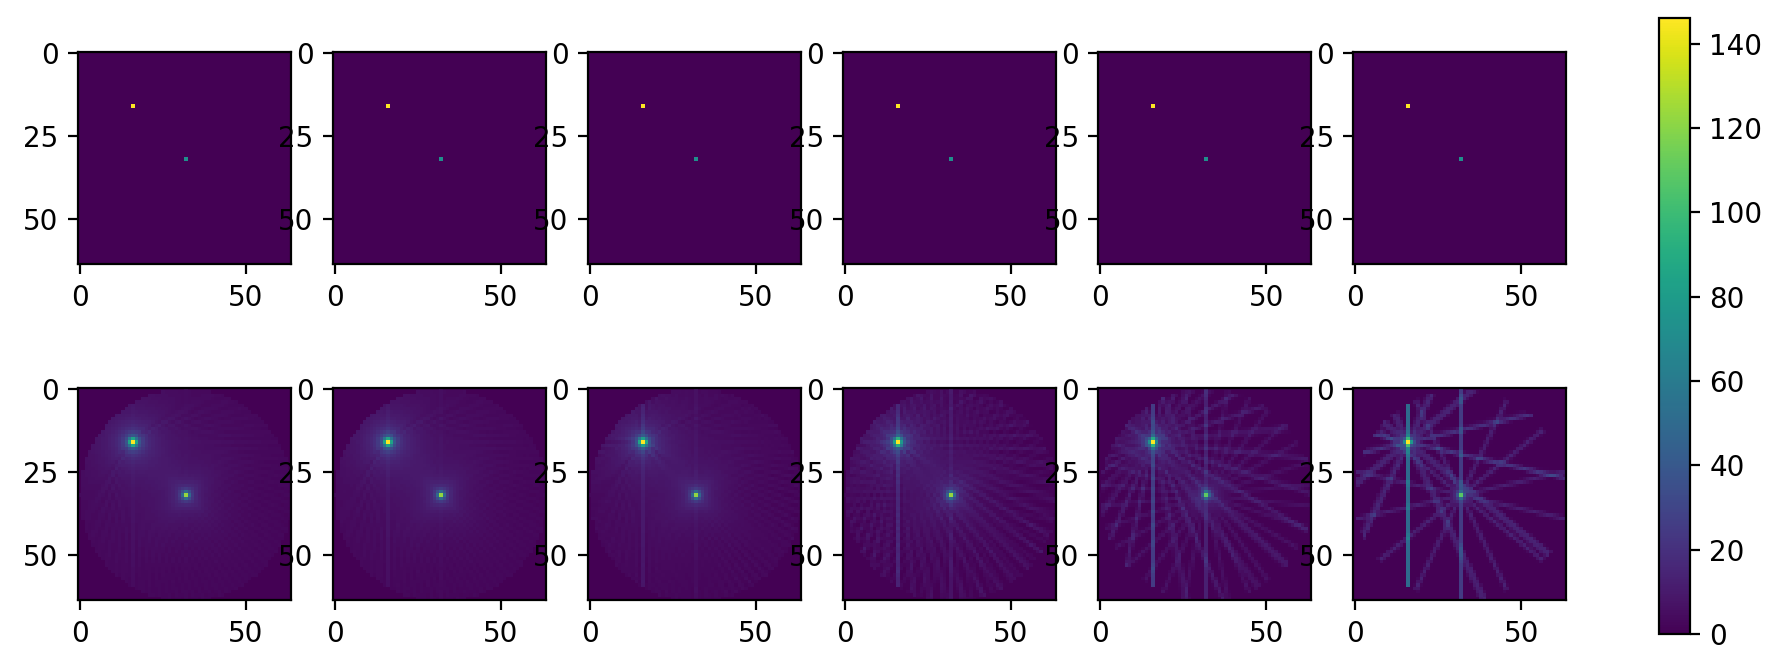
\includegraphics[width=\linewidth]{HW2_Q3_3.2.png}
    \caption{ Left to Right: N from 256 to 8.
        Top: original object image $f(r,c)$; middle: reconstructed object image $\widehat{f(r,c)}$; bottom: yellow region indicates the non-zero region in the reconstructed object image $\widehat{f(r,c)}\ne 0$.}
    \label{fig:recon}
\end{figure}

\begin{table}[!htp]
\centering
\begin{tabular}{c||c|c}
    \hline
     & Pt1 peak width & Pt2 peak width\\
    \hline
    N=256 & 1.62 & 2.56\\
    N=128 & 1.62 & 2.58\\
    N=64  & 1.61 & 2.48\\
    N=32  & 1.63 & 2.84\\
    N=16  & 1.66 & 2.97 \\
    N=8   & 1.51 & 3.62 \\
    \hline
\end{tabular}
\caption{Peak width at Point 1 (32,32) and Point 2 (16,16)}
\label{tab:err}
\end{table}

\begin{figure}[!htp]
    \centering
    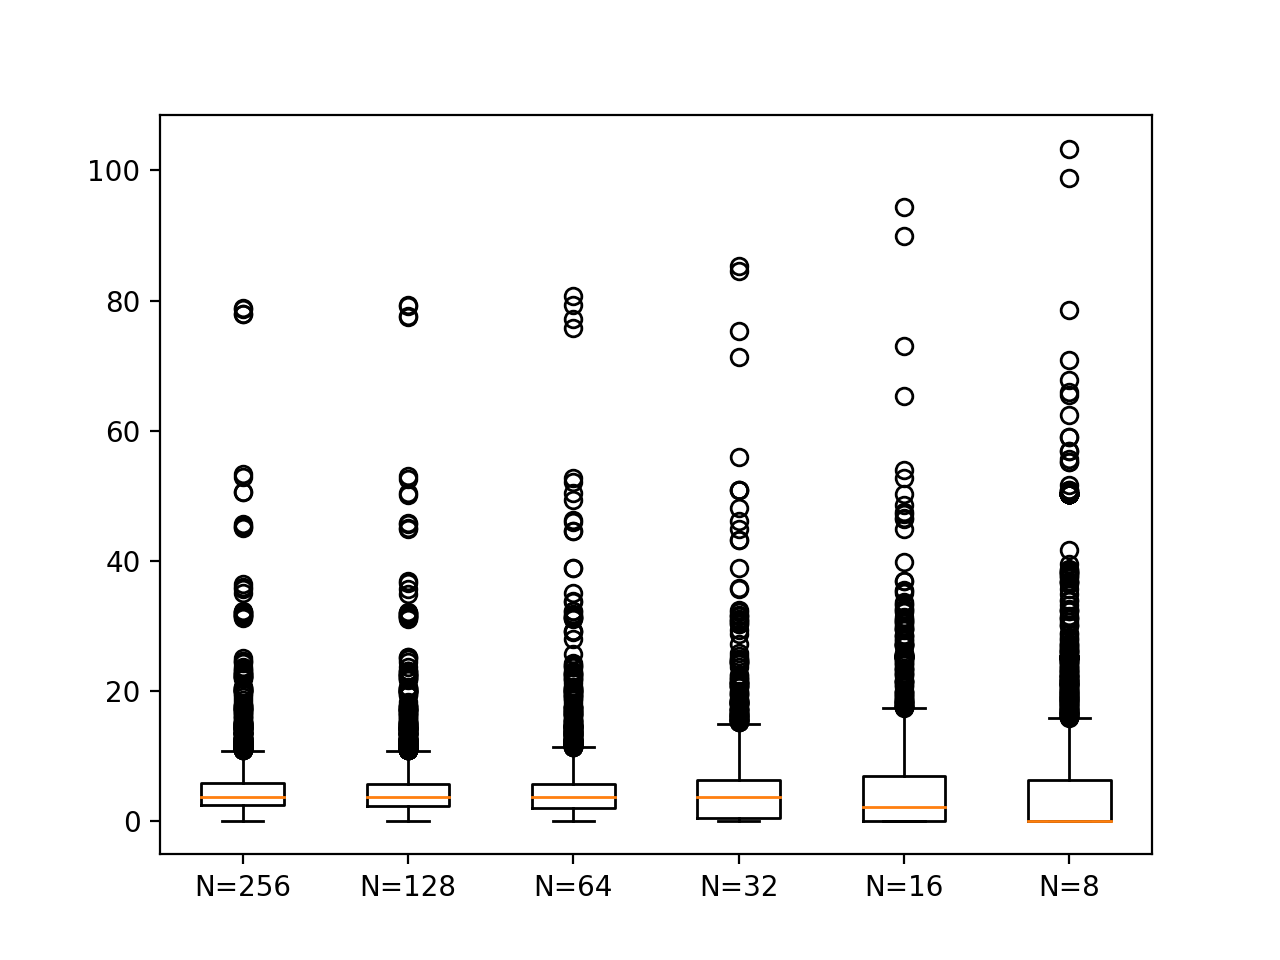
\includegraphics[width=0.8\linewidth]{HW2_Q3_3.3.png}
    \caption{Boxplot of reconstruction error.}
    \label{fig:boxplot}
\end{figure}

As we can see in figure ~\ref{fig:sino}, when N decreases, the sinogram curve seems to be discrete. And so as the reconstructed object image ~\ref{fig:recon}. As shown in figure ~\ref{fig:boxplot}, we analyze the error distribution and find that the mean error remains almost same while the error variance and maximum increases as N decreases. As shown in table ~\ref{tab:err}, smaller N causes larger peak widths on reconstructed images. So larger N should be preferred for multiple object imaging to reduce reconstruction errors. 

\textbf{d.}
\begin{figure}[!htp]
    \centering
    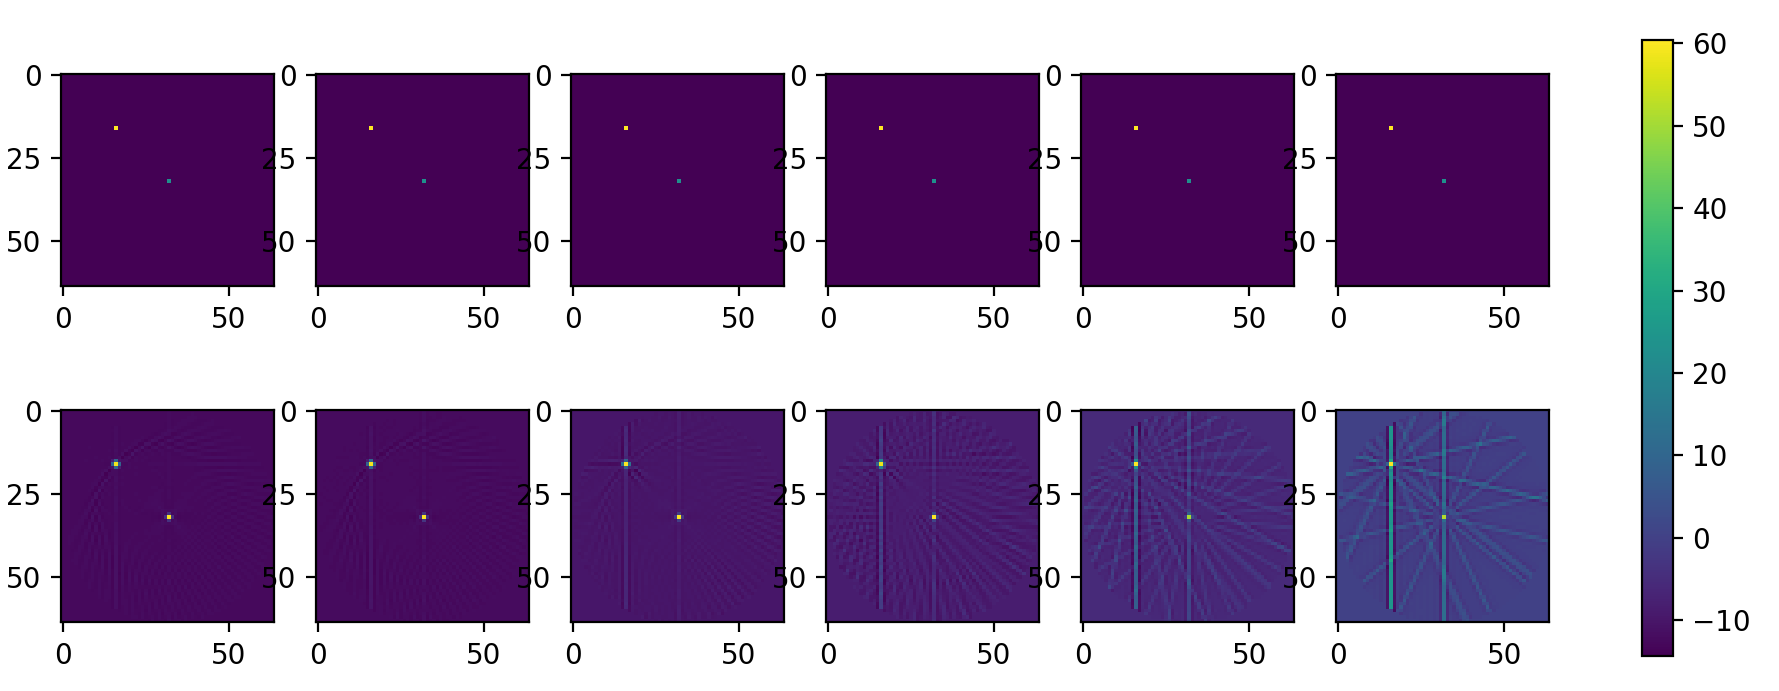
\includegraphics[width=\linewidth]{HW2_Q3_4.1.png}
    \caption{Left to right: N from 256 to 8.
        Top: original object image $f(r,c)$; middle: reconstructed object image $\widehat{f(r,c)}$ via ramp filter; bottom: yellow region indicates the non-zero region in the reconstructed object image $\widehat{f(r,c)}\ne 0$.}
    \label{fig:recon2}
\end{figure}

% \vspace{-2cm}
\begin{table}[!htp]
    \centering
    \begin{tabular}{c||c|c}
        \hline
        & Pt1 peak width & Pt2 peak width\\
        \hline
        N=256 & 1.15 & 1.46\\
        N=128 & 1.15 & 1.47\\
        N=64  &  1.15 & 1.38\\
        N=32 &  1.18 & 1.69\\
        N=16 & 1.21 & 1.74 \\
        N=8  & 1.08 & 2.13 \\
        \hline
    \end{tabular}
    \caption{Peak width at Point 1 (32,32) and Point 2 (16,16) when using Ramp filter}
    \label{tab:err_ramp}
    \end{table}

\begin{figure}[!htp]
    \centering
    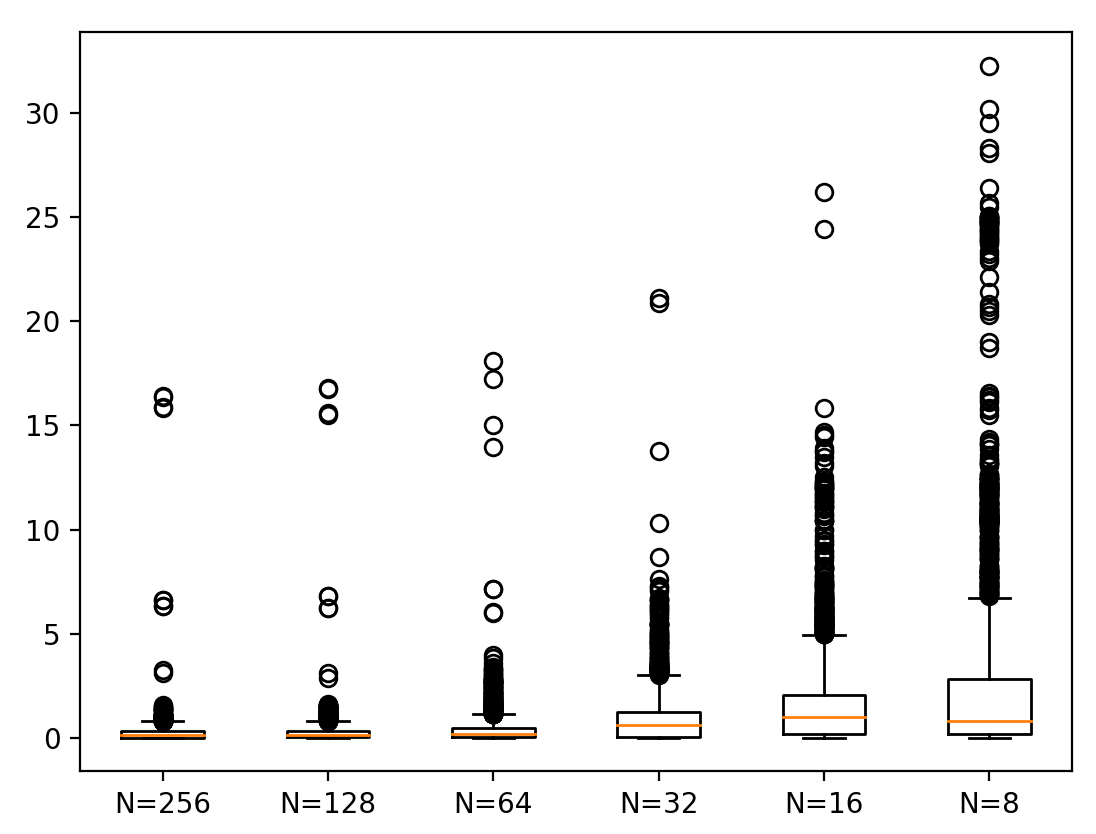
\includegraphics[width=0.8\linewidth]{HW2_Q3_4.2.png}
    \caption{Boxplot of reconstruction error.}
    \label{fig:boxplot2}
\end{figure}

As shown in figure ~\ref{fig:recon2} and ~\ref{fig:boxplot2}, the results show that using Ramp filter could reduce reconstruction error, especially when the number of views N is large. 

\newpage 
\qtitle{Ex4}
For rect function, \\
\begin{equation}
    rect(x) = 
      \begin{cases}
        1 & |x| \le k_{max}\\
        0 & otherwise
      \end{cases}       
  \end{equation}

For triangle funciton, \\
\begin{equation}
    triang(x) = 
      \begin{cases}
        k_{max}+x & -k_{max}\le x \le 0\\
        k_{max}-x & 0 < x \le k_{max} \\
        0 & otherwise
      \end{cases}       
\end{equation}

\begin{equation}
    RL(x) = rect(x)-triang(x) = 
      \begin{cases}
        |x| & |x| \le k_{max}\\
        0 & otherwise
      \end{cases}       
\end{equation}

In spatial domain, apply inverse Fourier transform, \\
$RL_g(\omega)=\mathcal{F}^{-1}(RL(t))=\bint{-\infty}{\infty}RL(t)exp(i2\pi \omega t)dt\\
=(\bint{-k_{max}}{0}(-t) exp(i2\pi \omega t)dt + \bint{0}{k_{max}}(t) exp(i2\pi \omega t)dt)\\
=exp(i2\pi\omega t)(i2\pi\omega t-1)/((i2\pi\omega)^2)\mid_{t=0}^{t=k_{max}}
+exp(i2\pi\omega t)(i2\pi\omega t-1)/((i2\pi\omega)^2)\mid_{t=-k_{max}}^{t=0}\\
=\cfrac{exp(i2\pi\omega k_{max})(i2\pi\omega k_{max}-1)+exp(-i2\pi\omega k_{max})(-i2\pi\omega k_{max}-1)+2}{-4\pi^2\omega^2}$

Use Euler's equation and simplify $k_{max}=k$, \\
$RL_g(\omega)=\cfrac{2\pi\omega k(2sin(2\pi k\omega))+2cos(2\pi k\omega)-2}{(2\pi \omega^2)}\\
=k^2(\cfrac{2sin(2\pi k\omega)}{2\pi k \omega}+\cfrac{-4sin(\pi k\omega)^2}{(2\pi k \omega)^2})\\
=k^2(2sinc(2\pi k\omega)-sinc(\pi k\omega)^2)$

\newpage
\qtitle{EX5}
\textbf{a.}
$f_d(x,y)=c(x,y)f(x,y)$. The diminished object looks like the following figure. 

\begin{figure}[!htp]
    \centering
    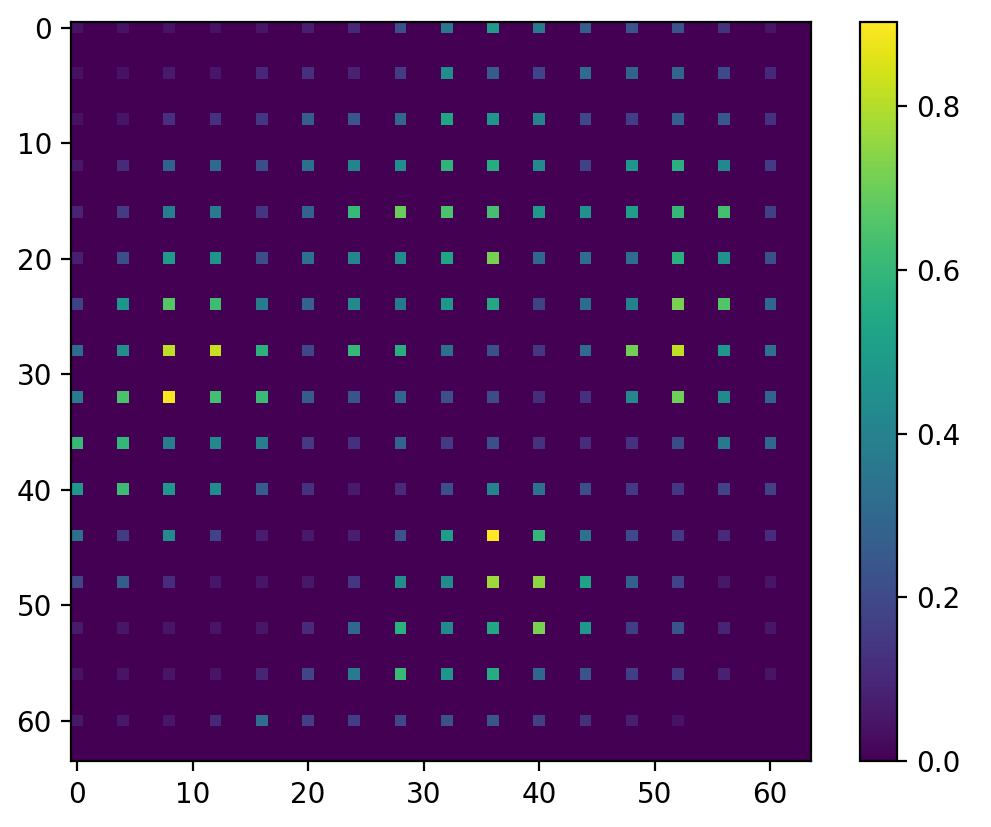
\includegraphics[width=0.6\linewidth]{HW2_Q5_1.png}
    \caption{Visualization of diminished f.}
    \label{fig:diminish}
\end{figure}

\textbf{b.}
Image $g(u,v)$ looks like: 

\begin{figure}[!htp]
    \centering
    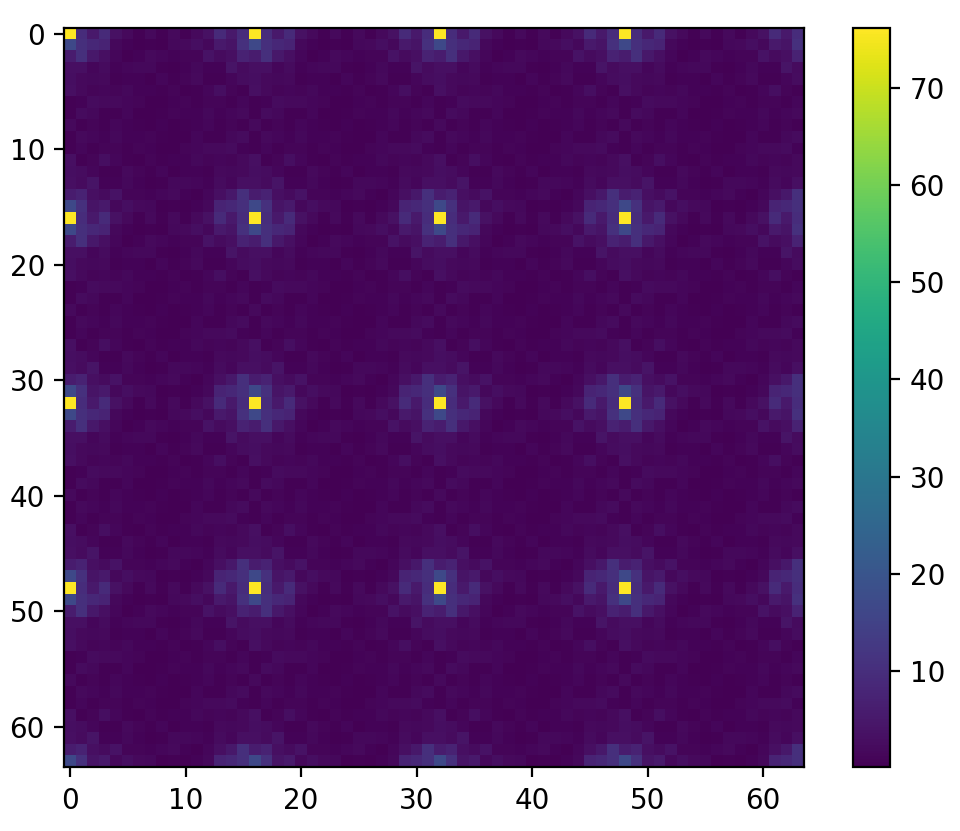
\includegraphics[width=0.6\linewidth]{HW2_Q5_2.png}
    \caption{Visualization of g(u,v).}
    \label{fig:g}
\end{figure}


\textbf{c.}
$\tilde{c}(u,v)=\mathcal{F}\{c(x,y)\}=\int\int c(x,y)exp(-i2\pi(ux+vy))dxdy\\
=\sum_{m=-\infty}^{\infty}\sum_{n=-\infty}^{\infty}exp(-i2\pi(uT_m+vT_n))$

As the following figure shows, $\tilde{c}$ is the comb filter on the u,v domain.

\begin{figure}[!htp]
    \centering
    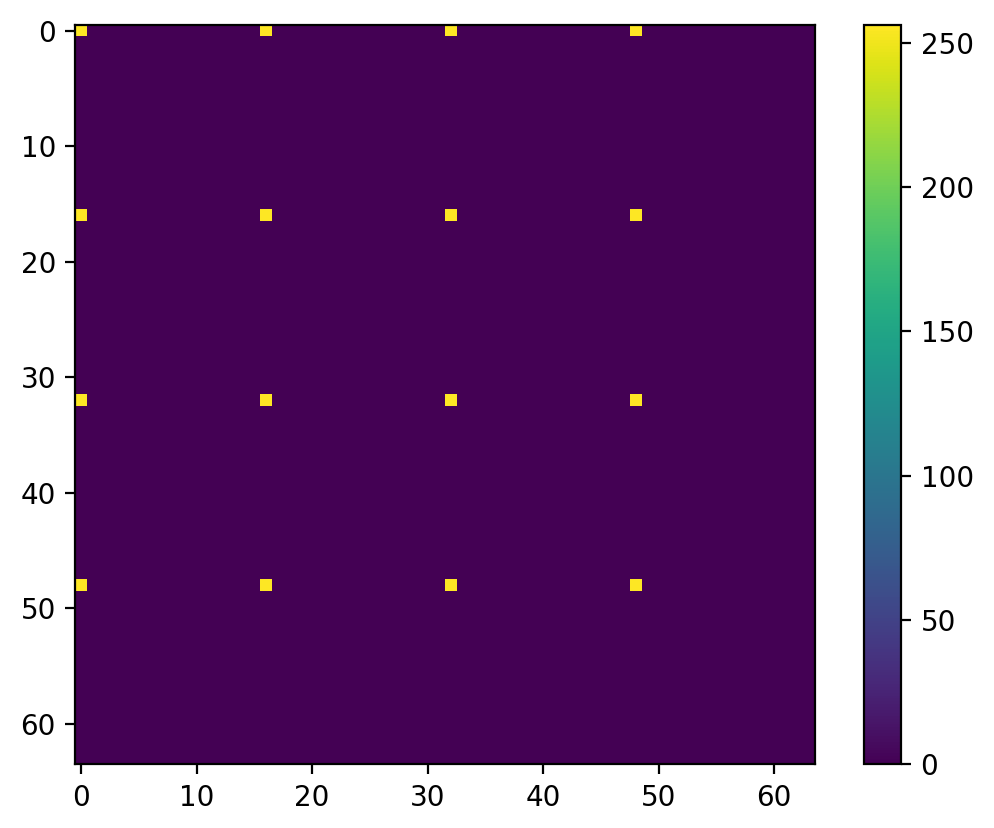
\includegraphics[width=0.6\linewidth]{HW2_Q5_3.png}
    \caption{Visualization of Fourier transformed c.}
    \label{fig:fc}
\end{figure}

\textbf{d.}
% Use convolve2d(g, fc, mode=same).
Let $g_d=np.multiply(g, d)$
\begin{figure}[!htp]
    \centering
    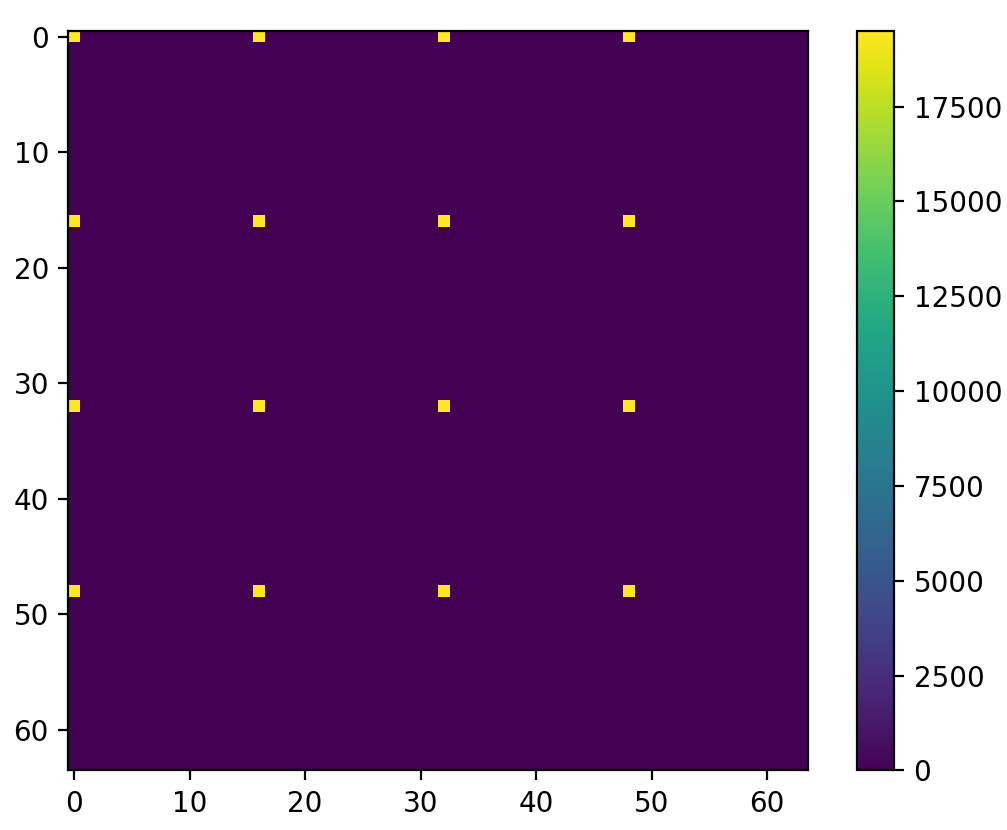
\includegraphics[width=0.6\linewidth]{HW2_Q5_4.2.png}
    \caption{Visualization of $g_d(u, v)$.}
    \label{fig:gd}
\end{figure}

\textbf{e.}
% $\mathcal{F}^{-1}[g_d(u, v)]\ne f_d(x,y)$. 
Since $f_d(x,y)$ is discrete and sparsely distributed, after Fourier transformation, it should distribute broadly on the transformed space. It means some information is saved beyond particular points, as figure ~\ref{fig:g} shows. So applying comb filter $\tilde{c}$ to g will lose these information, causing $g_d\ne g$. Therefore, $\mathcal{F}^{-1}g=f_d$, but $\mathcal{F}^{-1}g_d\ne f_d$ 


\begin{figure}[!htp]
    \centering
    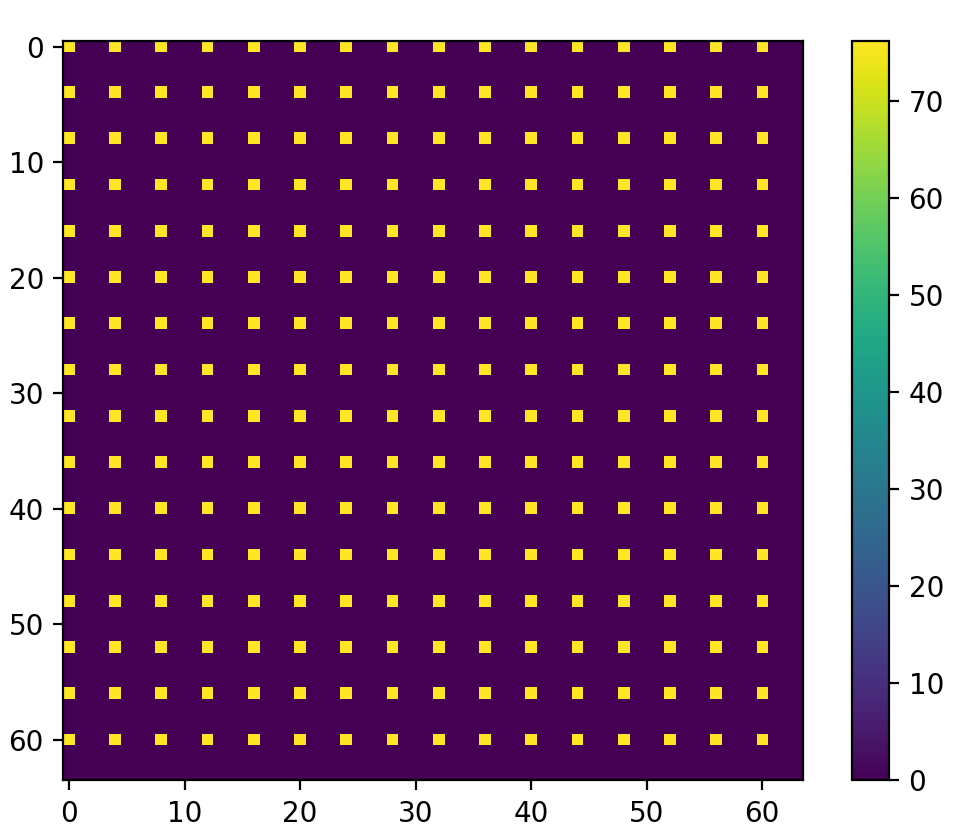
\includegraphics[width=0.6\linewidth]{HW2_Q5_5.2.png}
    \caption{Visualization of Fourier transformed g(u,v).}
    \label{fig:ifftgd}
\end{figure}

\begin{lstlisting}
    import cv2
    
    image = "hw01_ex08_HeLa-cells-from-imagej.png"
    img = cv2.imread(image)
    img = img / 255
    f = img[:,:, 0]
    h, w = f.shape
    c = np.zeros((h, w))
    c[0::4, 0::4] = 1
    # a. diminished f
    fd = f*c
    # b. fft g
    g = np.fft.fft2(fd)
    # c. fft c
    fc = np.fft.fft2(c)
    # d. gd
    gd = fc * g
    # e. igd
    igd = np.fft.ifft2(gd)
    igd = np.abs(igd)
    print(igd)
    
    plt.imshow(igd)
    plt.colorbar()
    plt.show()
\end{lstlisting}


\newpage
\qtitle{Ex6}
\textbf{a.} 
Let 
\begin{equation}
    circ(x, y) = \\
    \begin{cases}
        1 & x^2+y^2\le a^2\\
        0 & otherwise \\
    \end{cases}
\end{equation}

Since it'a 2-D Fourier transform, \\
$\widetilde{circ}(u, v)=\mathcal{F}\{circ(x, y)\}
=\infint\infint exp(-i2\pi (ux+vy))circ(x, y)dxdy$

Then transform to polar coordinates where \\ 
$x=rcos\theta,y=rsin\theta,u=\rho cos\varphi,v=\rho sin\varphi$,\\
$\widetilde{circ}(\rho, \theta)=\bint{a}{0}dr\bint{0}{2\pi}d\theta r exp(-i2\pi(r\rho cos\theta cos\varphi+ r\rho sin\theta sin \varphi))\\
=\bint{a}{0}dr\ r\bint{0}{2\pi}d\theta\ exp(-i2\pi r\rho cos(\theta-\varphi))$

\textbf{b.}
\begin{lstlisting}    
    def aperture(plane_size, pixel_size, aper_r):
        win_size = plane_size * pixel_size
        dk = np.arange(-win_size/2, win_size/2, pixel_size)
        xx, yy = np.meshgrid(dk, dk)
        plane = np.sqrt(xx**2+yy**2)
        print(plane)
        plane = np.where(plane>aper_r, 0, 1)
        return plane
    aper_rs = [1e-3,2e-3,4e-3]
    plane_size = 200 
    # set aper 
    R = 0.001
    pixel_size = 1e-4 # each pixel is 0.1mm

    fig, axs = plt.subplots(2, len(aper_rs))
    fig.set_size_inches(8, 5)
    for idx, aper_r in enumerate(aper_rs):
        plane = aperture(plane_size, pixel_size, aper_r)    
        # apply fft
        image = np.fft.fftshift(np.fft.fft2(plane))
        axs[0, idx].imshow(np.abs(plane), cmap="gray")
        axs[1, idx].imshow(np.abs(image), cmap="gray")
        axs[1,idx].set_xlabel('r={}'.format(aper_r))
    axs[0, 0].set_ylabel("circ")
    axs[1, 0].set_ylabel("F{circ}")
    plt.show()
\end{lstlisting}

\begin{figure}[!htp]
    \centering
    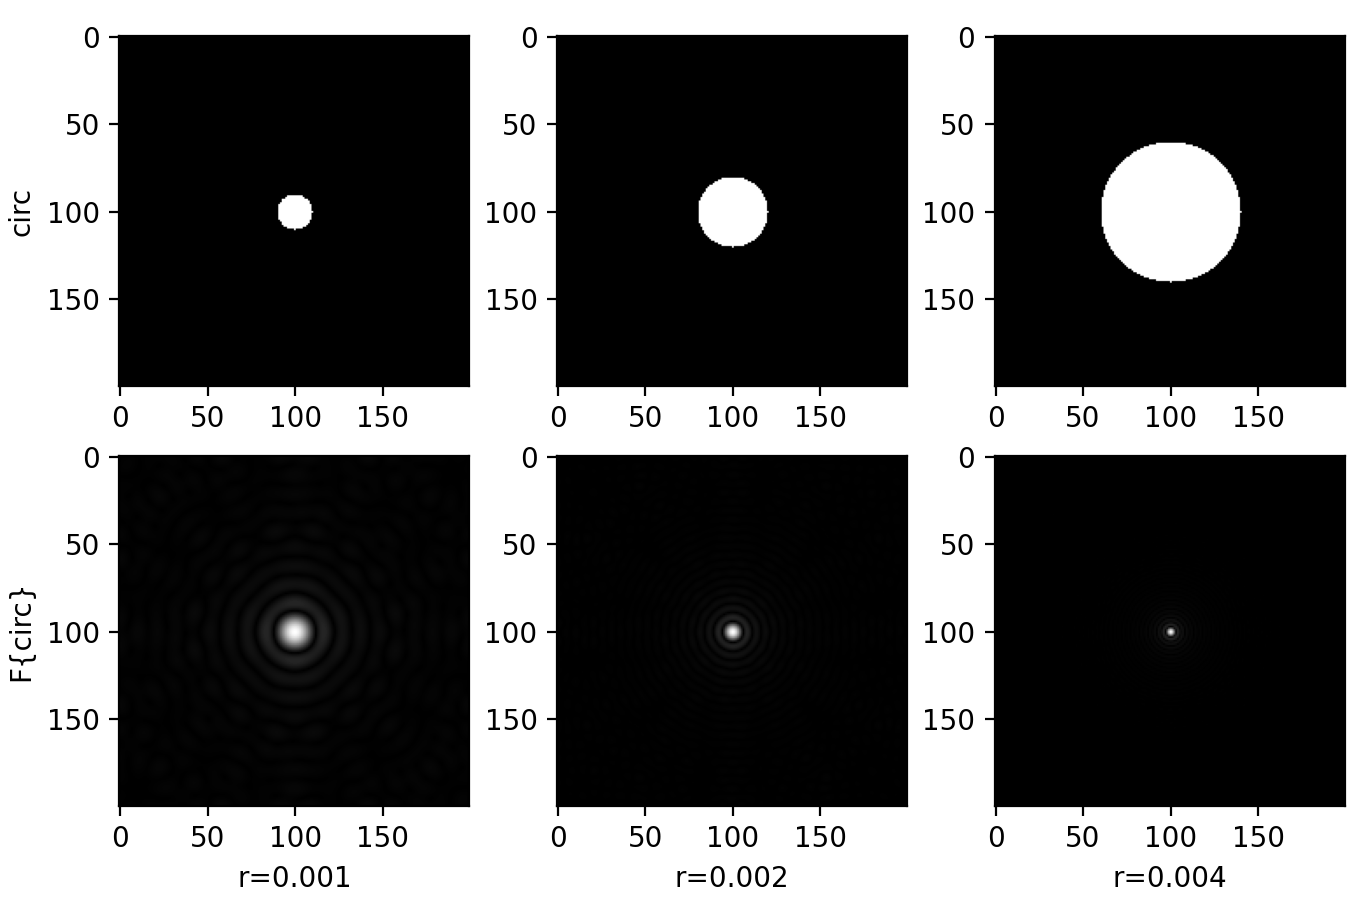
\includegraphics[width=\linewidth]{HW2_Q6_2.png}
    \caption{Visualization of Fourier transformed circular aperture with radius 1, 2, and 4 mm. Top row: circular aperture image $circ(x,y)$; Bottom row: Fourier transformed circular aperture $\mathcal{F}\{circ(x,y)\}$. }
    \label{fig:circ}
\end{figure}
As shown in figure~\ref{fig:circ}, as aperture radius increase, the imaging pixel intensities become more concentrated, which indicates the reduce diffraction effect in large aperture. 

\textbf{c.}
\begin{lstlisting}
    lam = 5e-7
    Z = 1
    detector_size = 32e-6
    num_detectors = 1024
    
    u = np.linspace(-1/2/detector_size, 1/2/detector_size, num_detectors)
    U,V = np.meshgrid(u, u)
    # fresnel approx
    H = np.exp(2j*np.pi/lam*Z)*np.exp(-1j*np.pi*lam*Z*(U**2+V**2)) 
    
    plane = aperture(plane_size, pixel_size, R)

    # Fourier Transform of the image
    O=np.fft.fft2(plane)
    # FFT shift
    Oshift=np.fft.fftshift(O)
    # multiply Fourier transform and propagator matrices.
    image=Oshift*H
    # inverse Fourier transform
    image=np.fft.ifft2(np.fft.ifftshift(image))
    
    plt.imshow(image.astype(np.float), cmap="gray")
    plt.show()
\end{lstlisting}

As seen in figure ~\ref{fig:aper10cm} and ~\ref{fig:aper100cm}, compared to $Z=10cm$, the aperture image obtained at $Z=100$ is more discrete. This is because diffraction make the energy distributed on larger area as the propagation distance increases.

\begin{figure}[htb]
\centering
\begin{minipage}{0.45\linewidth}
    % \begin{figure}
        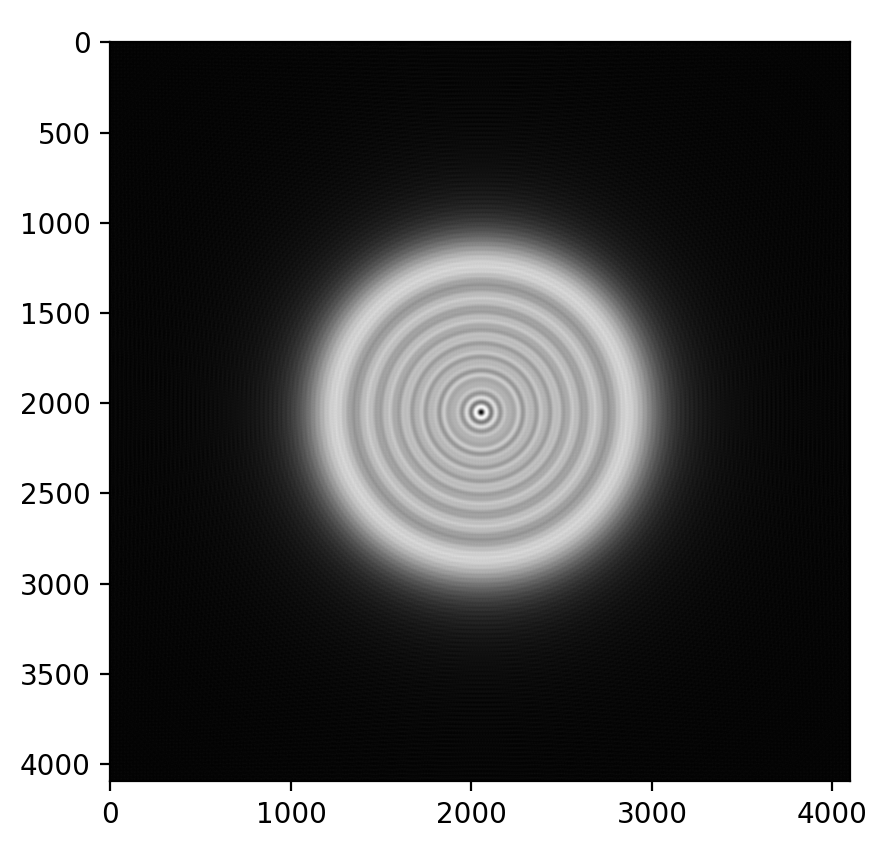
\includegraphics[width=\textwidth]{HW2_Q6_3.1.png}
        \caption{Aperture image at $Z=10cm$}
        \label{fig:aper10cm}
    % \end{figure}
\end{minipage}
\begin{minipage}{0.45\linewidth}
    % \begin{figure}
    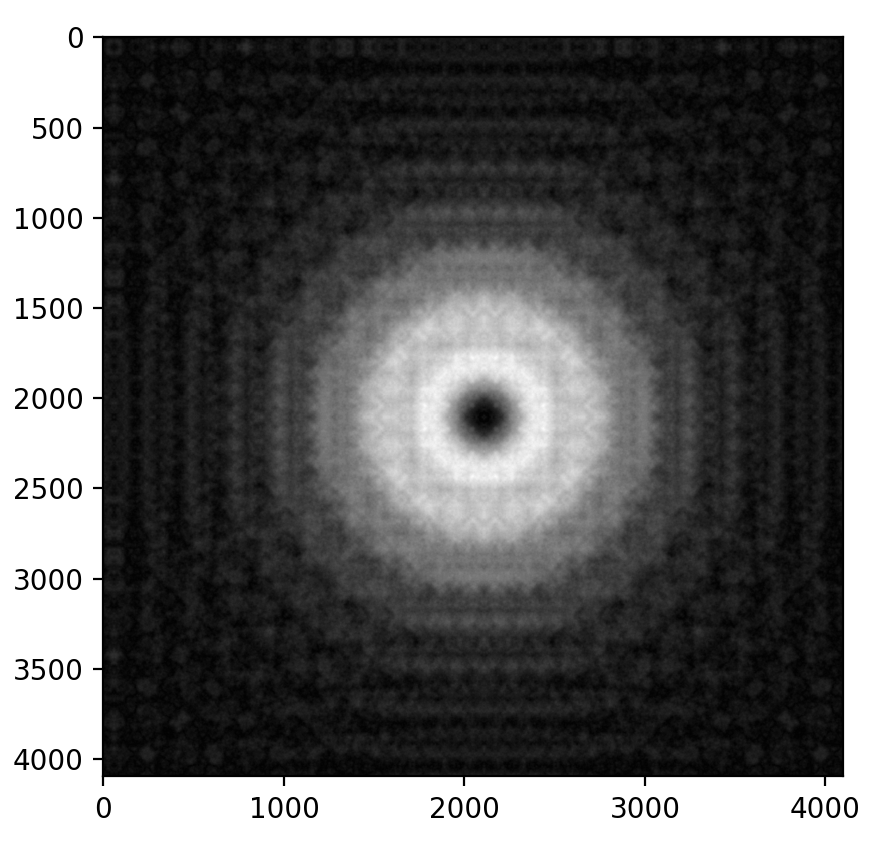
\includegraphics[width=\textwidth]{HW2_Q6_3.2.png}
    \caption{Aperture image at $Z=100cm$}
    \label{fig:aper100cm}
    % \end{figure}
\end{minipage}
\end{figure}

\textbf{d.}
Compared to continuous detector in c, the obtained object image via current detector seems to be smaller and less discrete, corresponding to the reduced resolution. 

\begin{figure}[htb]
    \centering
    \begin{minipage}{0.45\linewidth}
        % \begin{figure}
            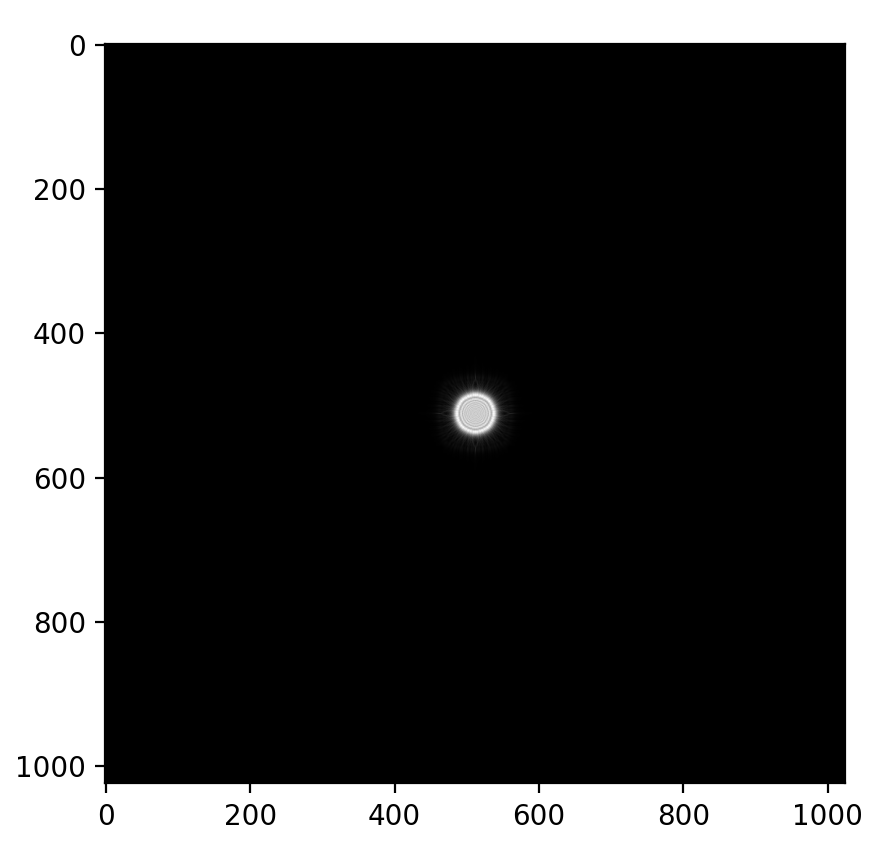
\includegraphics[width=\textwidth]{HW2_Q6_4.1.png}
            \caption{Aperture image at $Z=10cm$}
            \label{fig:disc_aper10cm}
        % \end{figure}
    \end{minipage}
    \begin{minipage}{0.45\linewidth}
        % \begin{figure}
        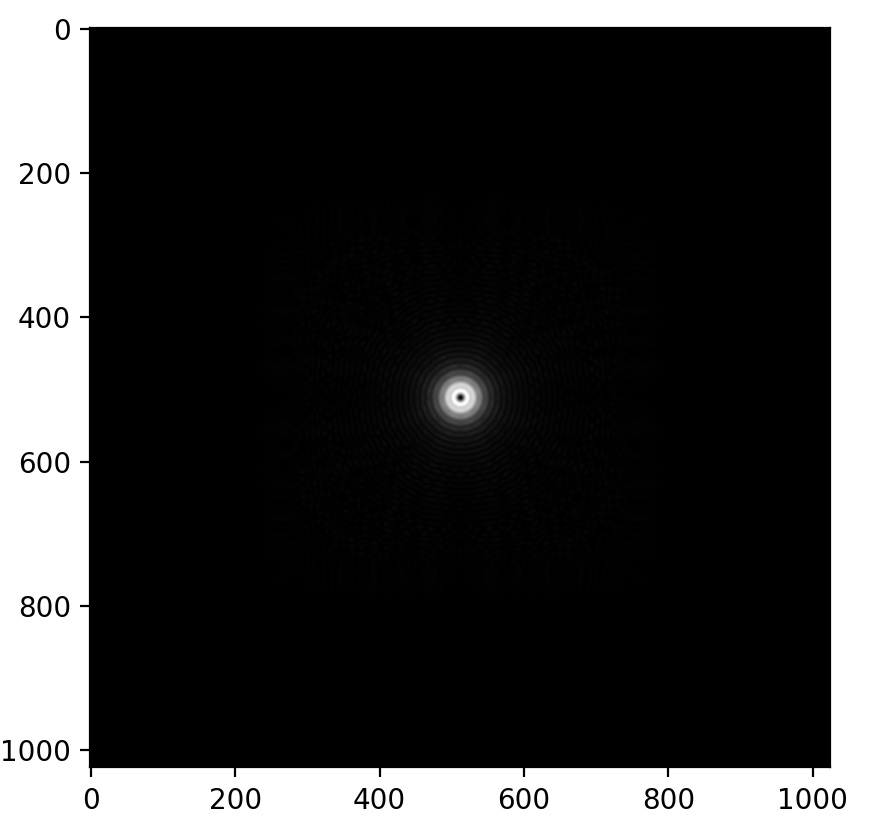
\includegraphics[width=\textwidth]{HW2_Q6_4.2.png}
        \caption{Aperture image at $Z=100cm$}
        \label{fig:disc_aper100cm}
        % \end{figure}
    \end{minipage}
    \end{figure}



\end{document}
